\section{NAND logic gate}
In this exercise the design of the NAND gate was expected to have minimum area while to have high fanout output(fanout =8). In order to find the delay time between input and output of the NAND gate, the Elmore Delay model~\cite{elmore1948transient} was used in the design.\\
\subsection{Design and Optimization}
As shown in the Figure~\ref{fig:nand}, NAND gate is constructed by two parallel connected PMOS transistors and two serial connected NMOS transistors. 

\begin{figure*}[ht]
\centering
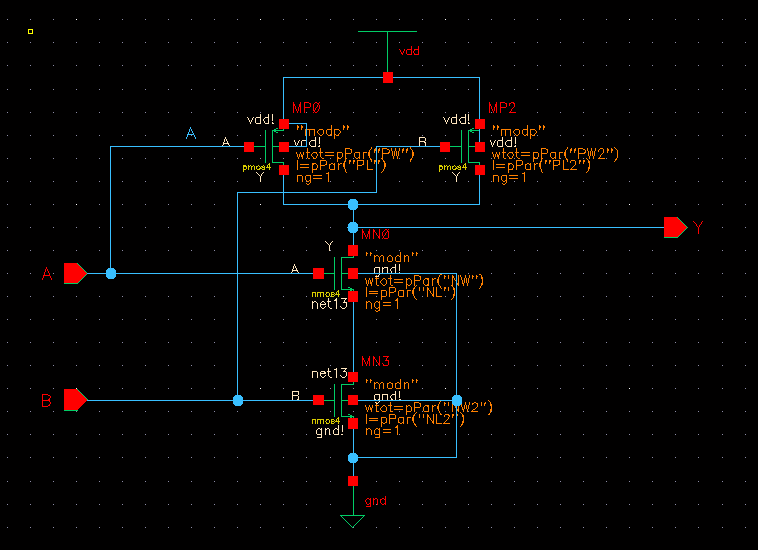
\includegraphics[width = 0.7\textwidth]{Figures/nand}
\caption{NAND gate schematic}
\label {fig:nand}
\end{figure*}

Although transistors have complicate current-voltage behaviour, turned on transistors can be assumed as resistors, a chain of transistors can be represented as an RC ladder, as shown in Figure~\ref{fig:elmore}. Therefore the Elmore delay model can estimate the delay of this RC ladder in terms of the path resistance and capacitance of a node on the ladder and the supply:

\begin{align}
	{t\textsubscript{pd} = \sum_{\substack{i}} R\substack{n-i}C\substack{i}}
\end{align}

\begin{figure}[H]
		\centering
		%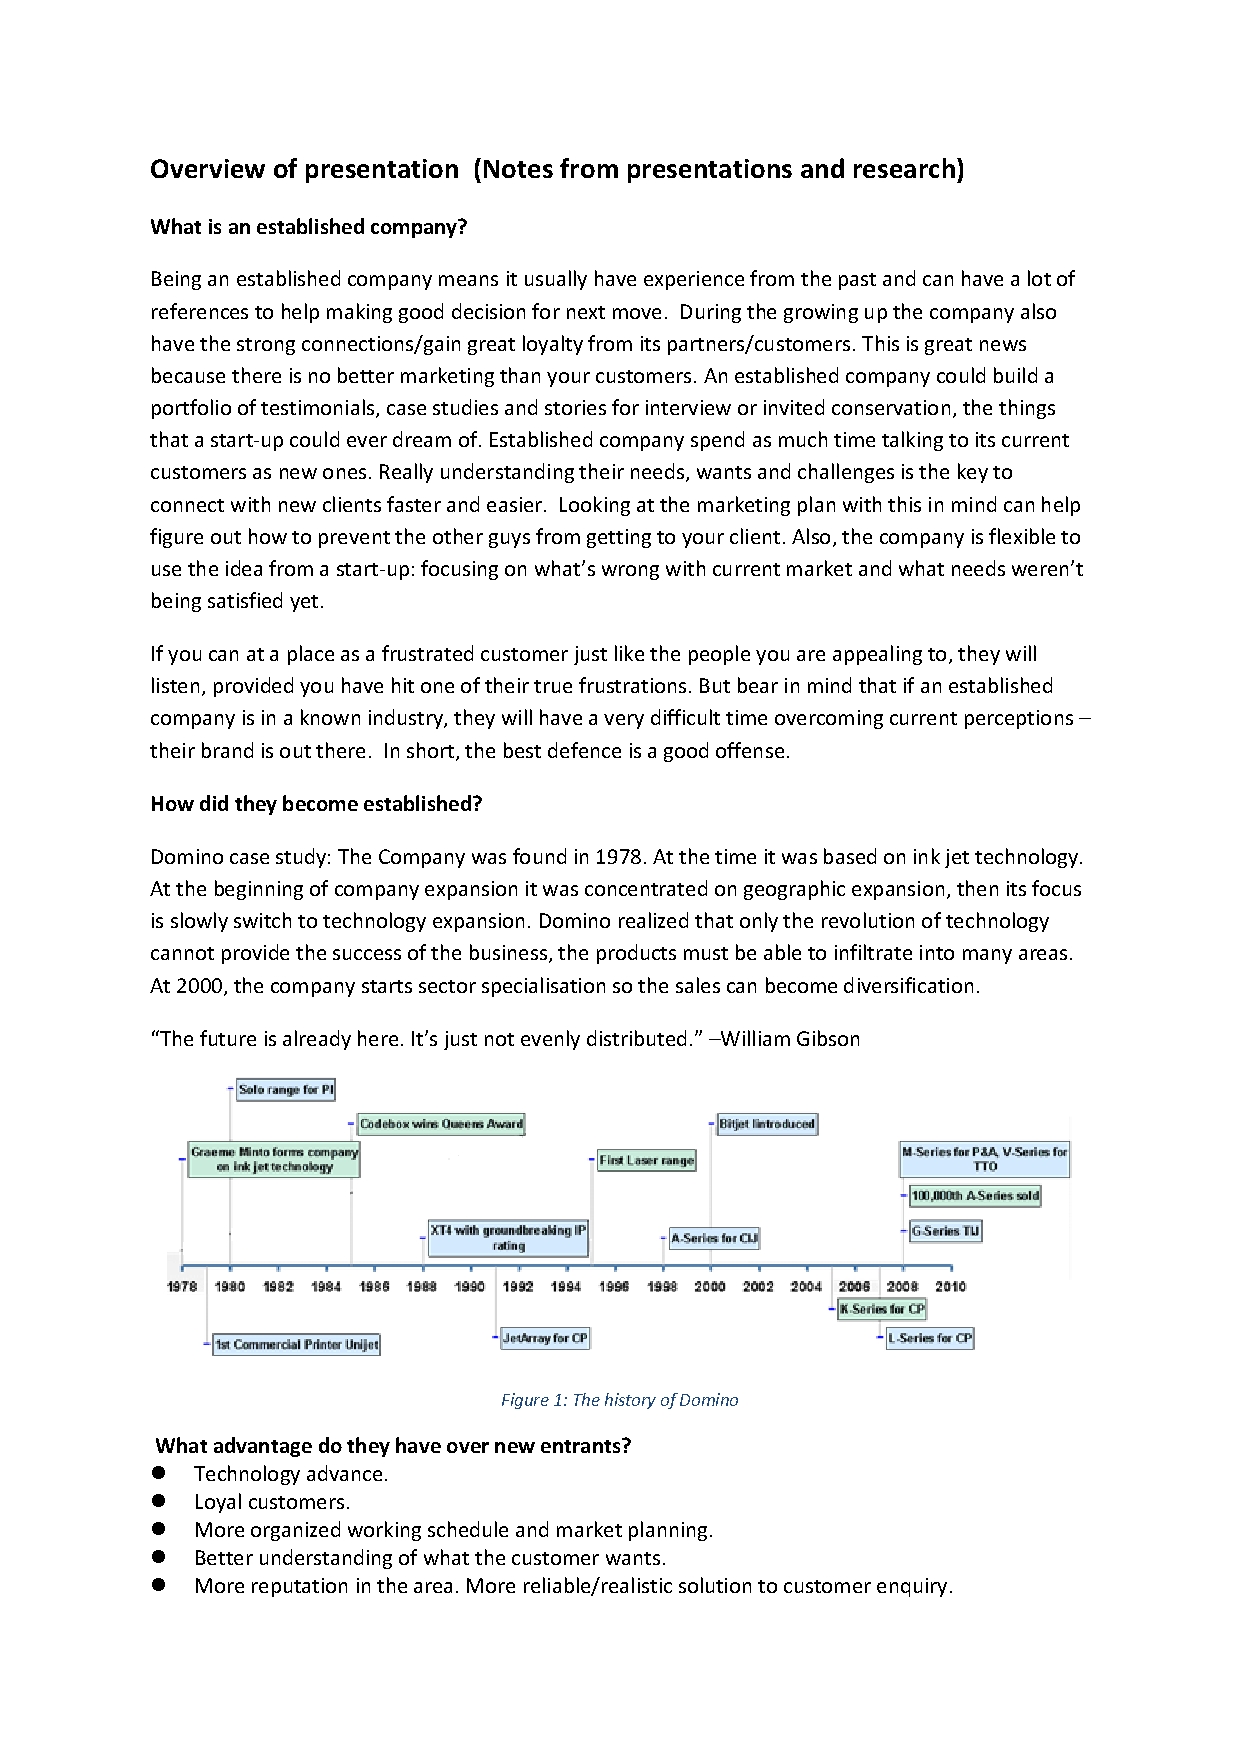
\includegraphics[width = 0.9\textwidth]{Figures/Overview_of_presentations}
		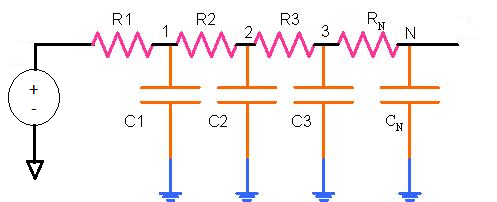
\includegraphics[width = 0.45\textwidth]{Figures/elmoredelaymodel}		
		\caption{Simple Elmore delay model}
		\label {fig:elmore}
\end{figure}
Therefore it is possible to use this method as the reference to calculate the width of logic gate, since the propagation delay is dependent to it and the capacitance of the load. \\
Typically in the logic gate, for parallel connected  transistors, the total resistance is lower when they are all on. In many gates, the worst-case delay is usually because only on the parallel transistor is on~\cite{[2]}. So when applying the Elmore delay model in the NAND design, one of input is connected to vdd while the other one is connected in the path, as shown in Figure~\ref{fig:nandtest}.
\begin{figure}[H]
		\centering
		%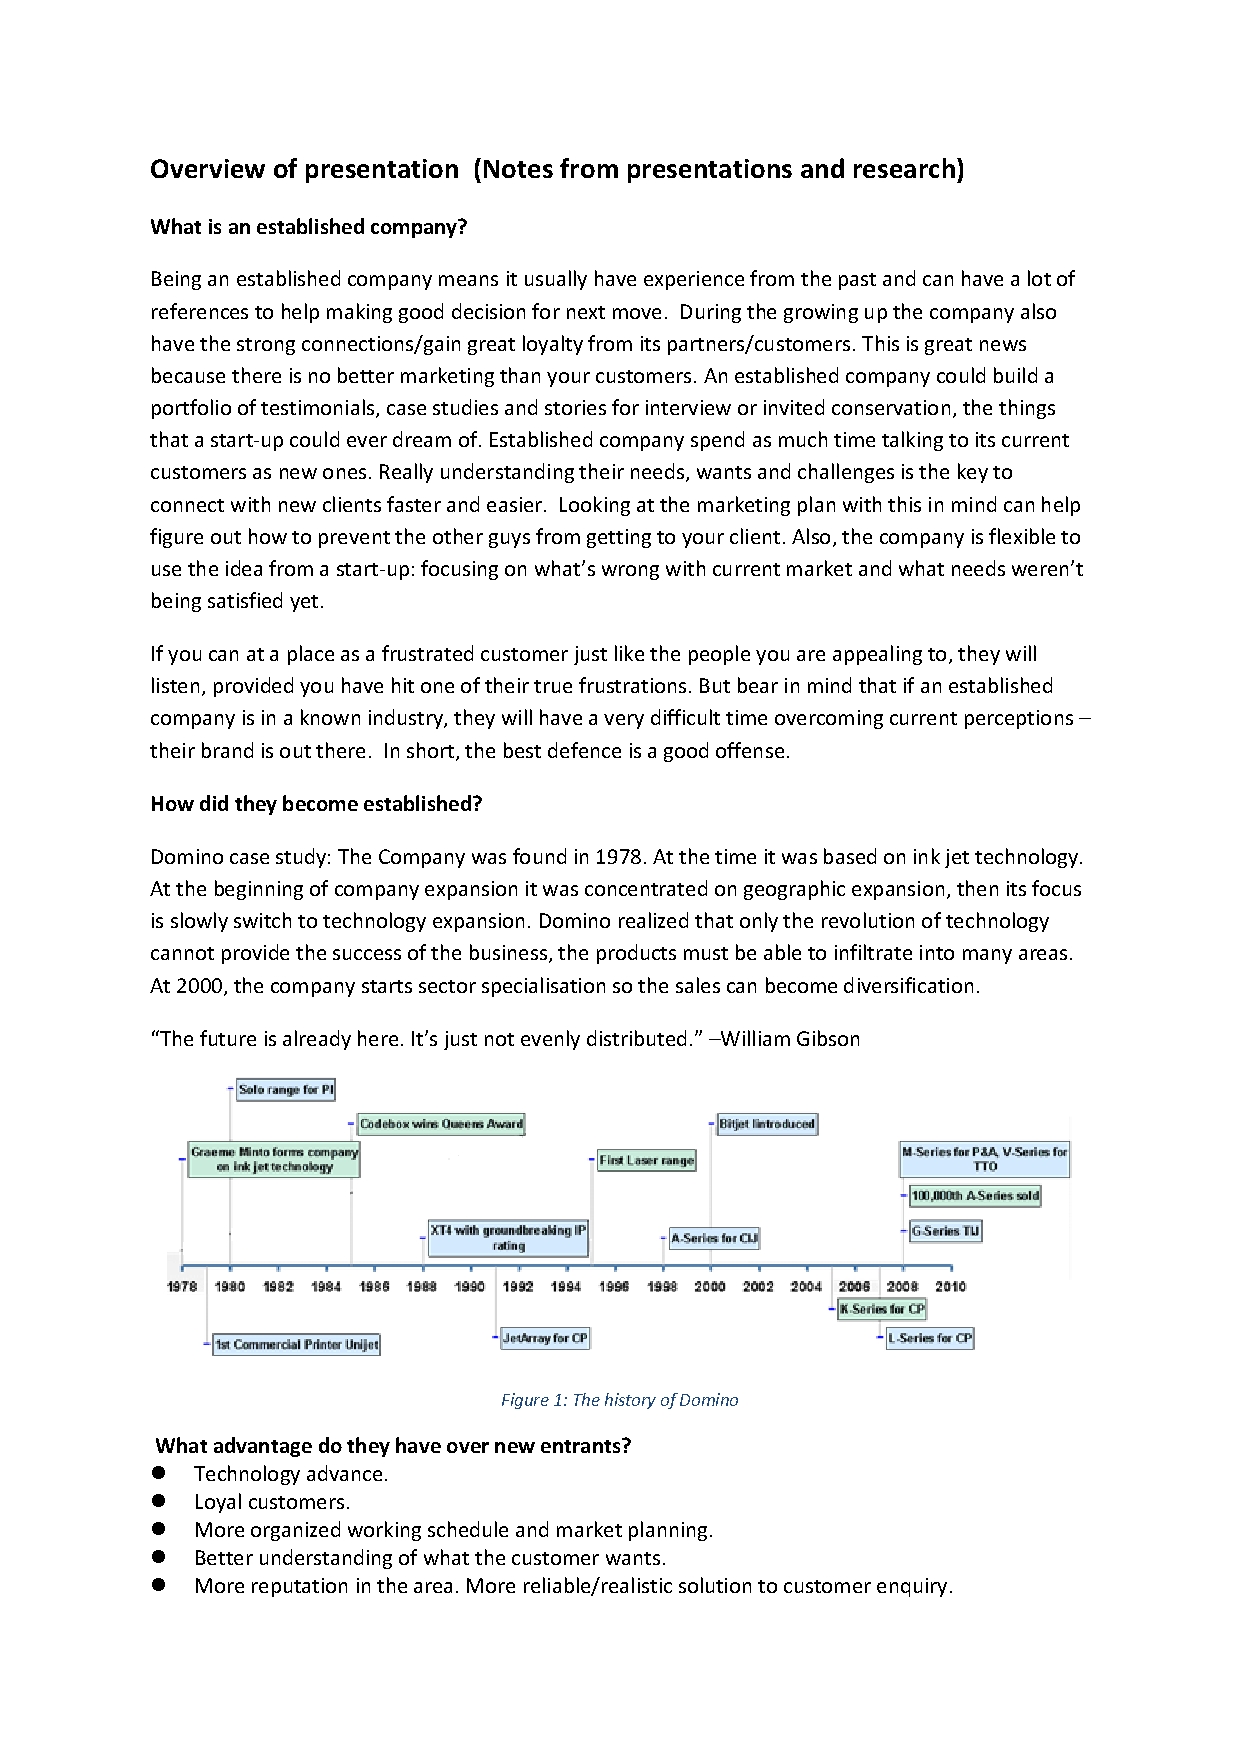
\includegraphics[width = 0.9\textwidth]{Figures/Overview_of_presentations}
		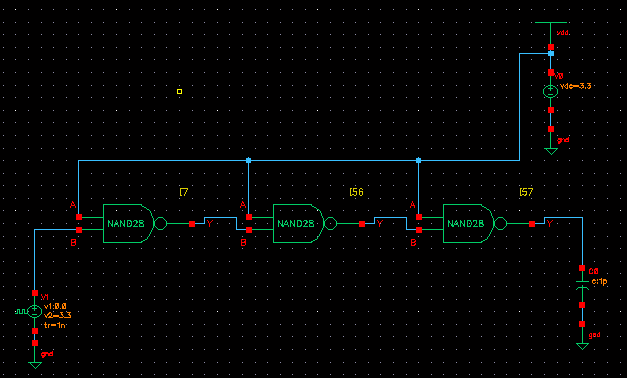
\includegraphics[width = 0.5\textwidth]{Figures/nandtest}		
		\caption{NAND Elmore delay model}
		\label {fig:nandtest}
\end{figure}

While deceasing the width of NMOS and increasing the width of PMOS, the propagation delays, which is the maximum time from input to output crossing 50\%, of the rising edge and falling edge are also changing. When the certain ratio between the width of PMOS and NMOS is reached, the propagation delay between rising edge and falling edge of logic gate will become similar. In another word, the signal slope at the output of logic gate will become quite identical to the input, only with an amount of delay.\\
In this design, the ratio between PMOS and NMOS is  at 2.3, as found in the Figure~\ref{fig:NANDratio}.
\begin{figure}[hf]
		\centering
		%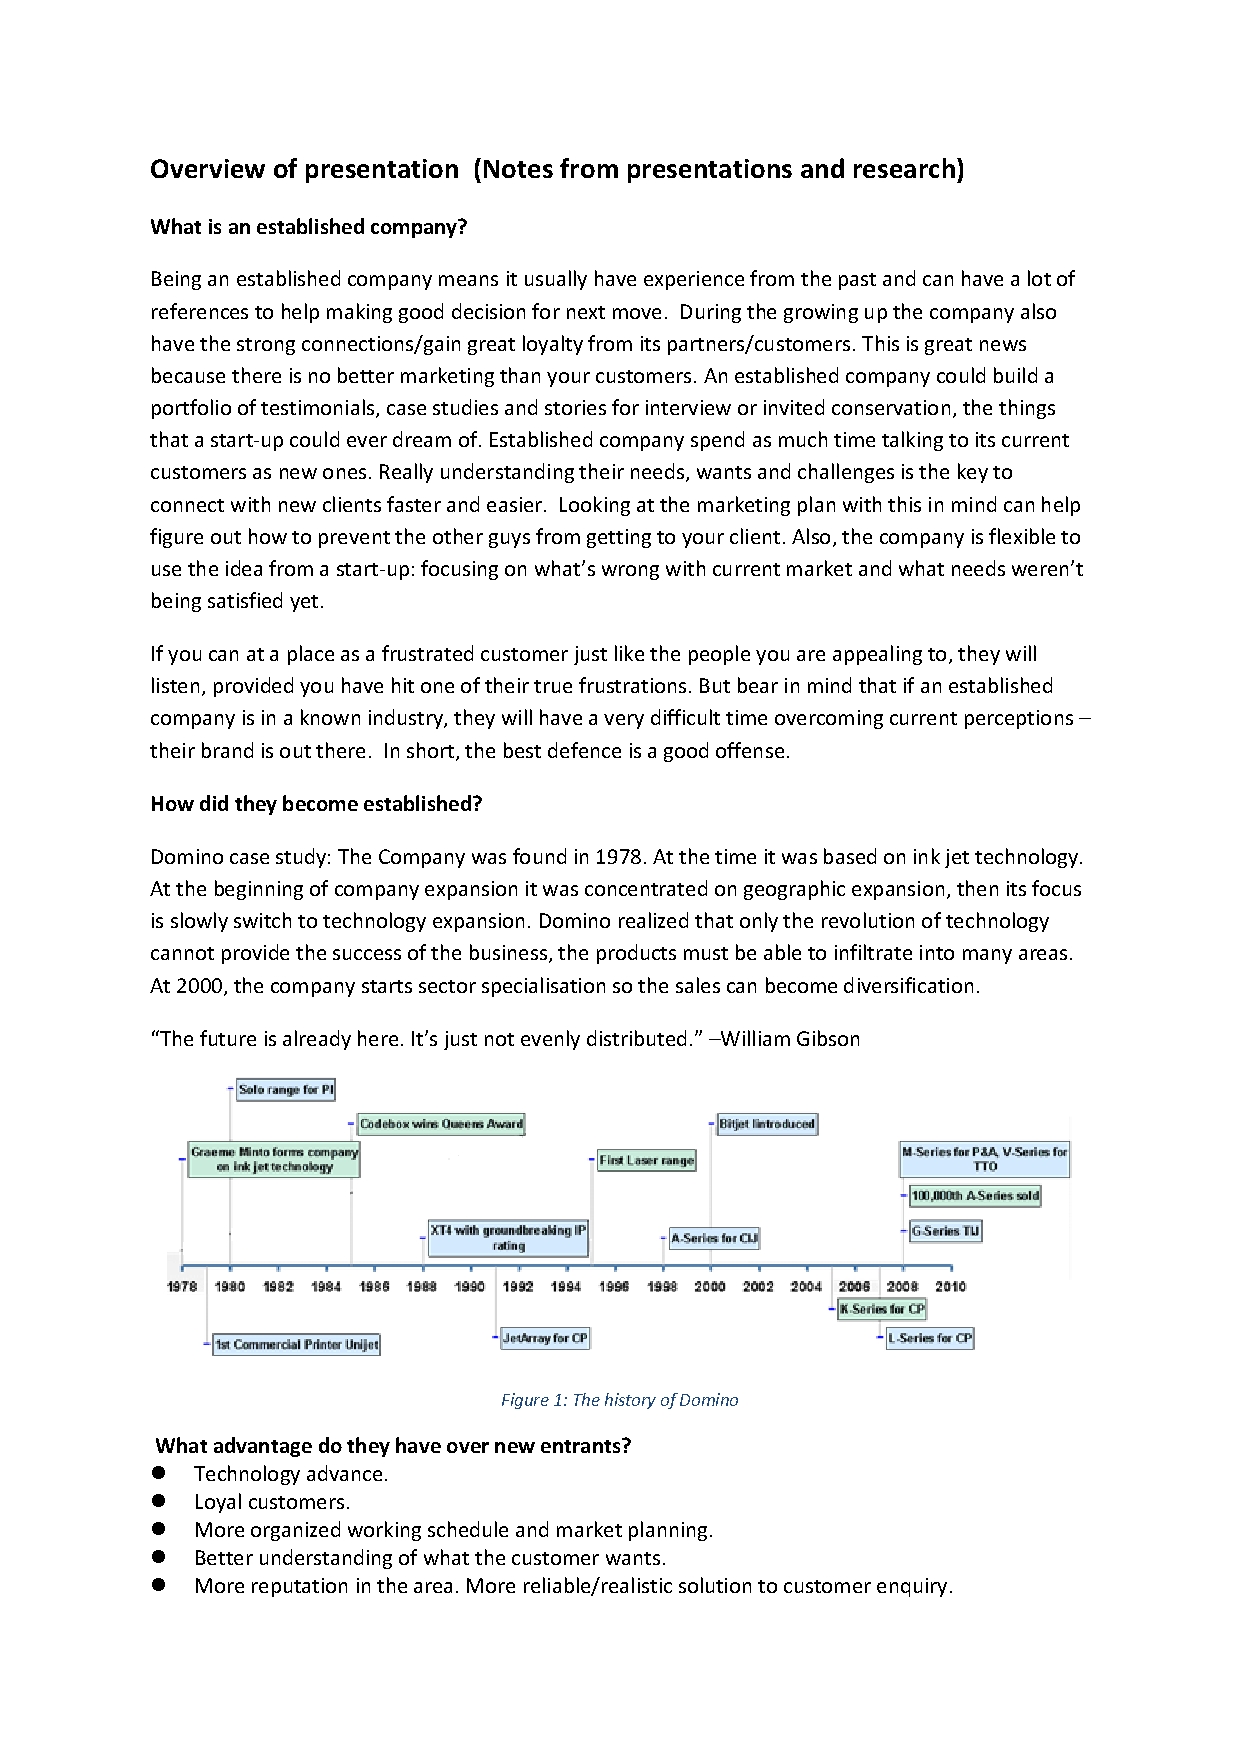
\includegraphics[width = 0.9\textwidth]{Figures/Overview_of_presentations}
		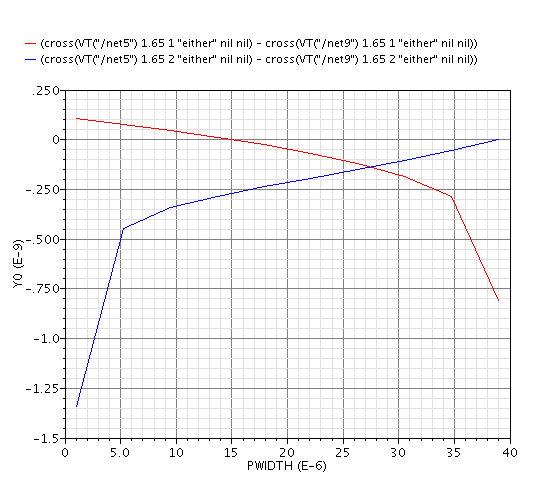
\includegraphics[width = 0.5\textwidth]{Figures/NANDratio}		
		\caption{Ratio of width of PMOS and NMOS in NAND gate}
		\label {fig:NANDratio}
\end{figure}

If a gate can drive n copies of itself, then it is said to have a fanout or electrical effort of n. When multiple gates are chain connected together, they could form a multi-stage logic network, the logical effort of logic gate is independent of size of next connected gate but the electrical effort is not. Therefore the ratio between size of PMOS and NMOS found previously is still legitimate for the design, but it is possible to find the speed of logic gate with fanout by using the multi-stage logic network gate.\\
A multi-stage logic network can be easily converted into a ring oscillator, which is often used as a process monitor to judge if a logic gate is fast or not. As shown in the Figure~\ref{fig:nandro}, the NAND gate is connected in serial to construct a ring oscillator, with 8 fanout gate attached to each stage.
\begin{figure*}[hf]
		\centering
		%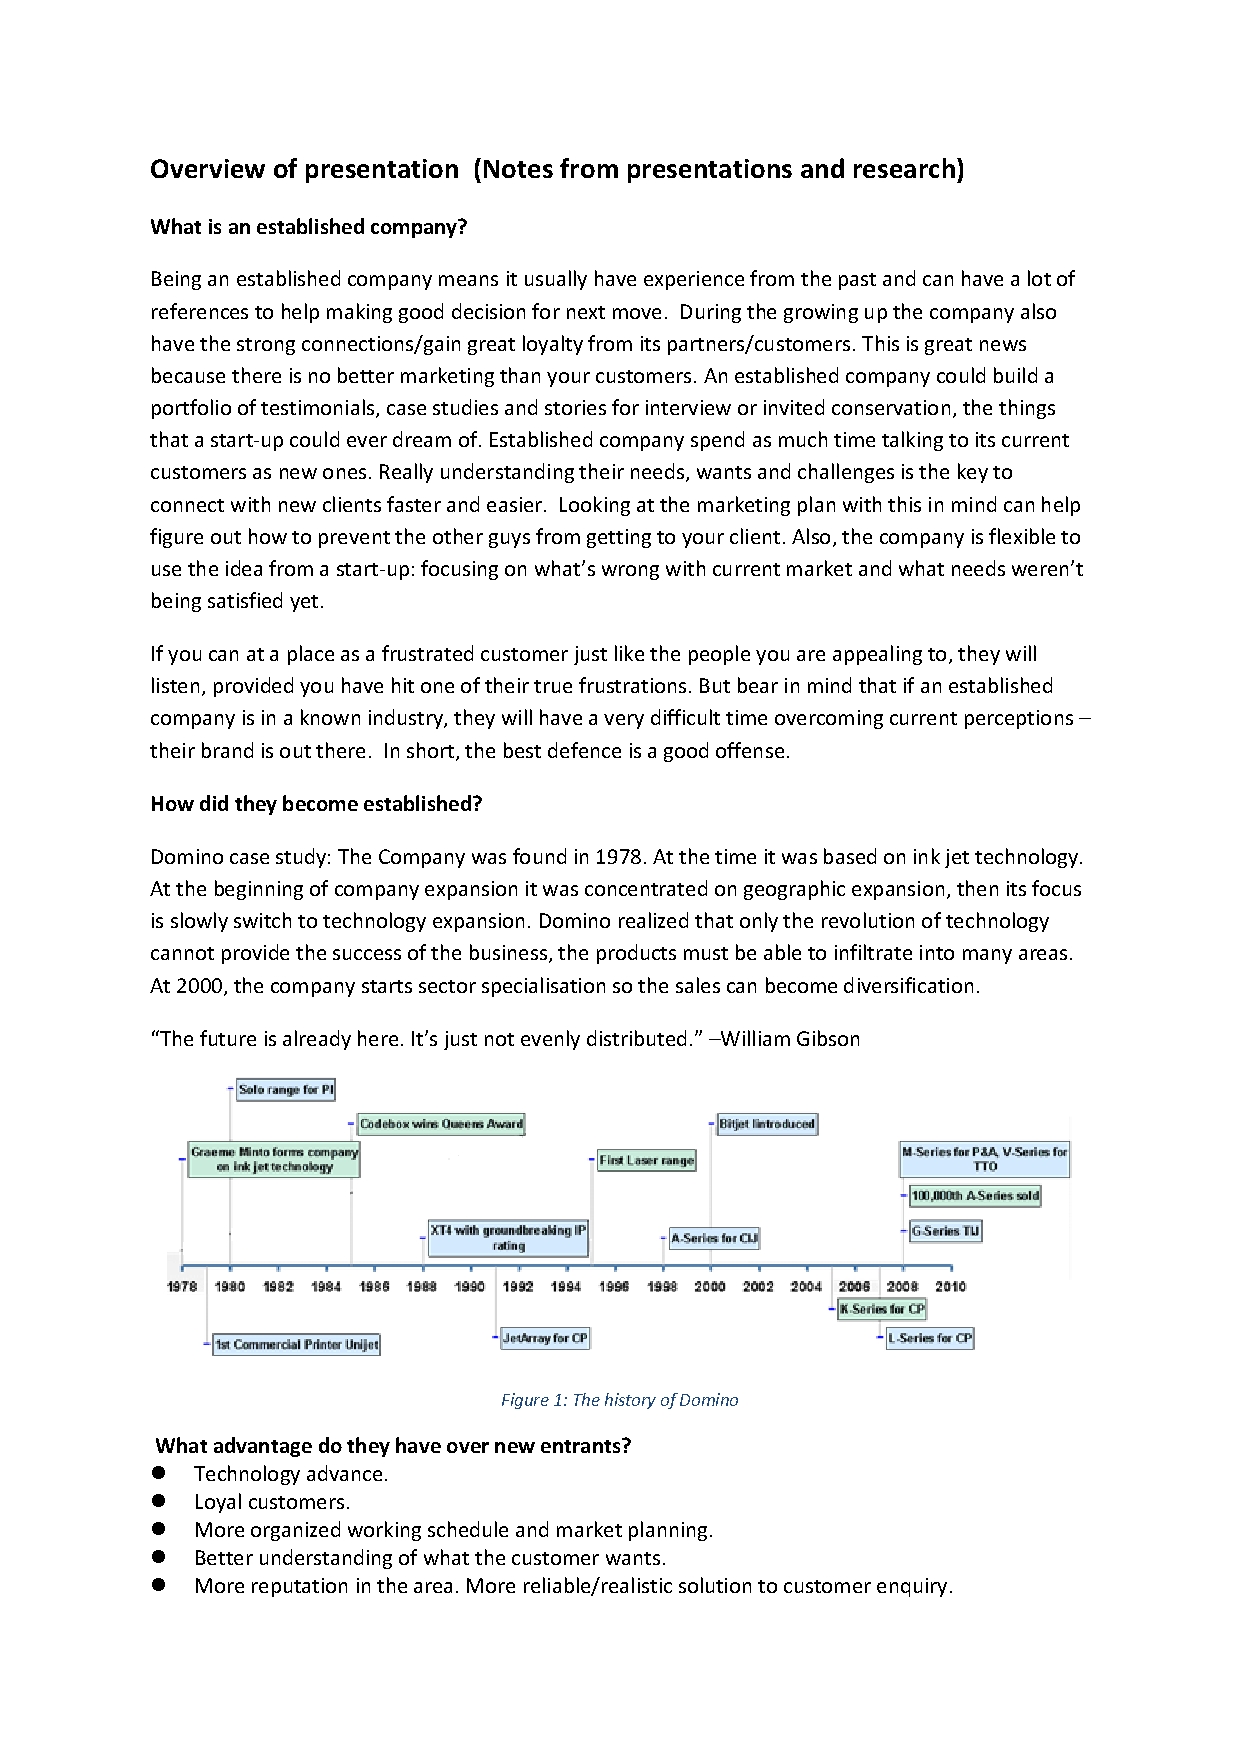
\includegraphics[width = 0.9\textwidth]{Figures/Overview_of_presentations}
		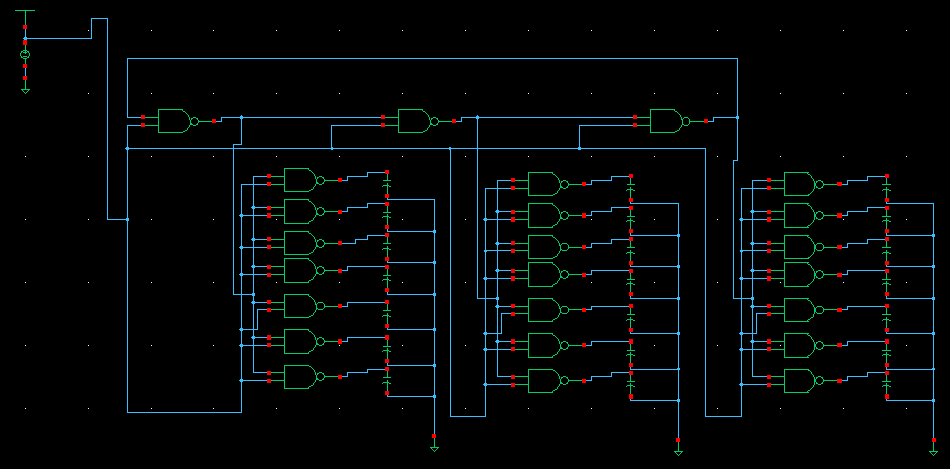
\includegraphics[width = 0.7\textwidth]{Figures/nandro}		
		\caption{NAND ring oscillator with fanout 8}
		\label {fig:nandro}
\end{figure*}

According to the frequency diagram obtained in Figure~\ref{fig:nandfreq}, the width of NMOS is set at 2.4um to achieve small area design without too much performance degradation.
\begin{figure}[hf]
		\centering
		%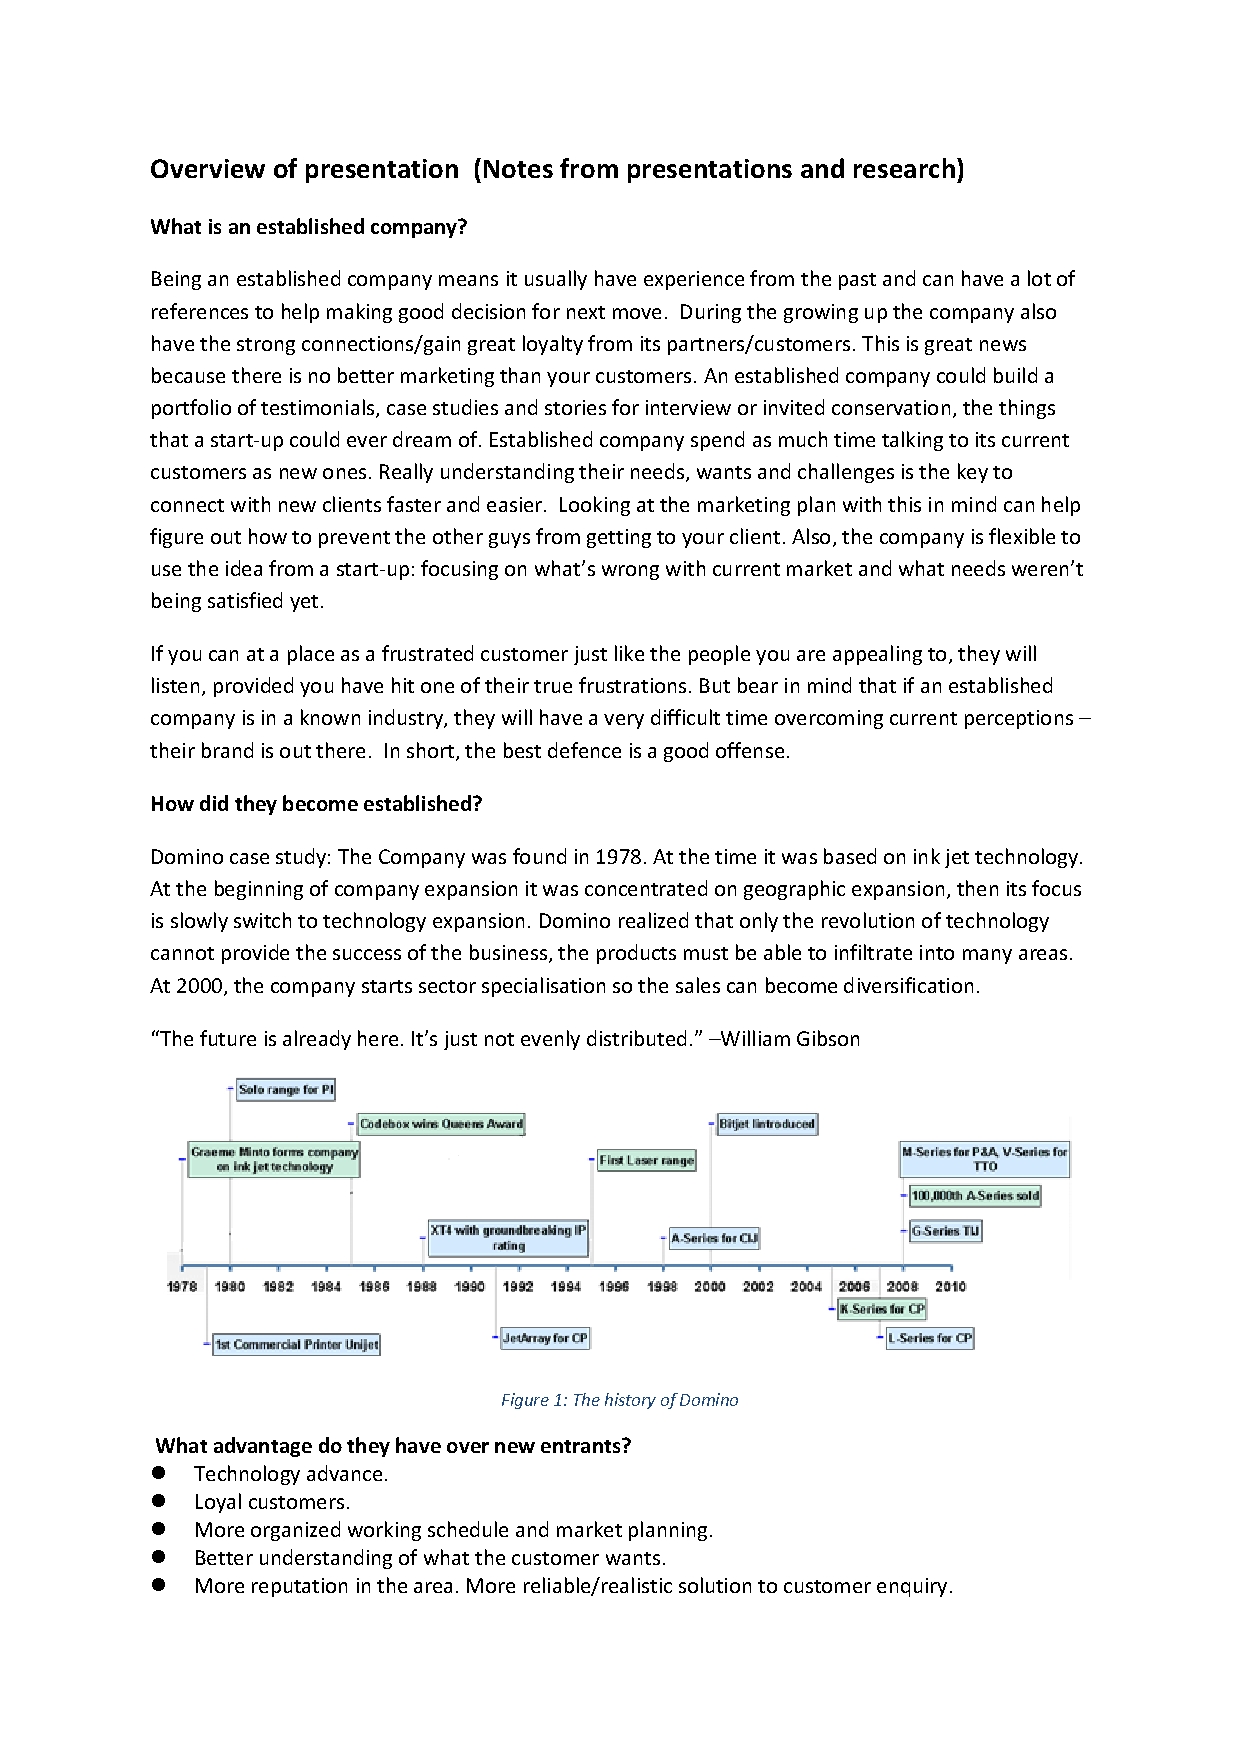
\includegraphics[width = 0.9\textwidth]{Figures/Overview_of_presentations}
		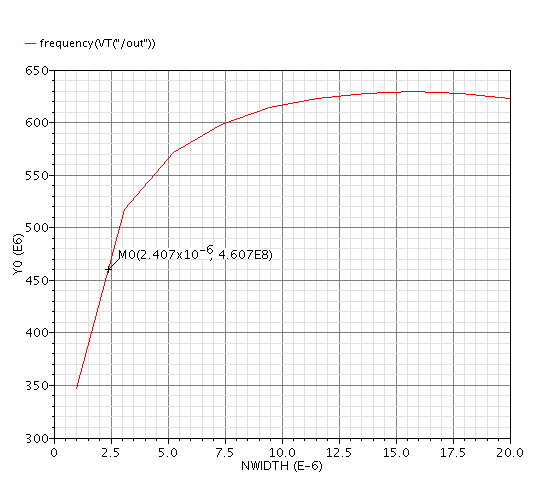
\includegraphics[width = 0.5\textwidth]{Figures/nandfreq}		
		\caption{Frequency of NAND gate in the Ring Oscillator}
		\label {fig:nandfreq}
\end{figure}

\subsection{Testing}
To the functionality of the design, two vpulse sources were used. One of input pulses has twice the period than another one so all possible input combinations can be generated, as shown in the Figure~\ref{fig:nandtest1}
   
\begin{figure*}[hf]
		\centering
		%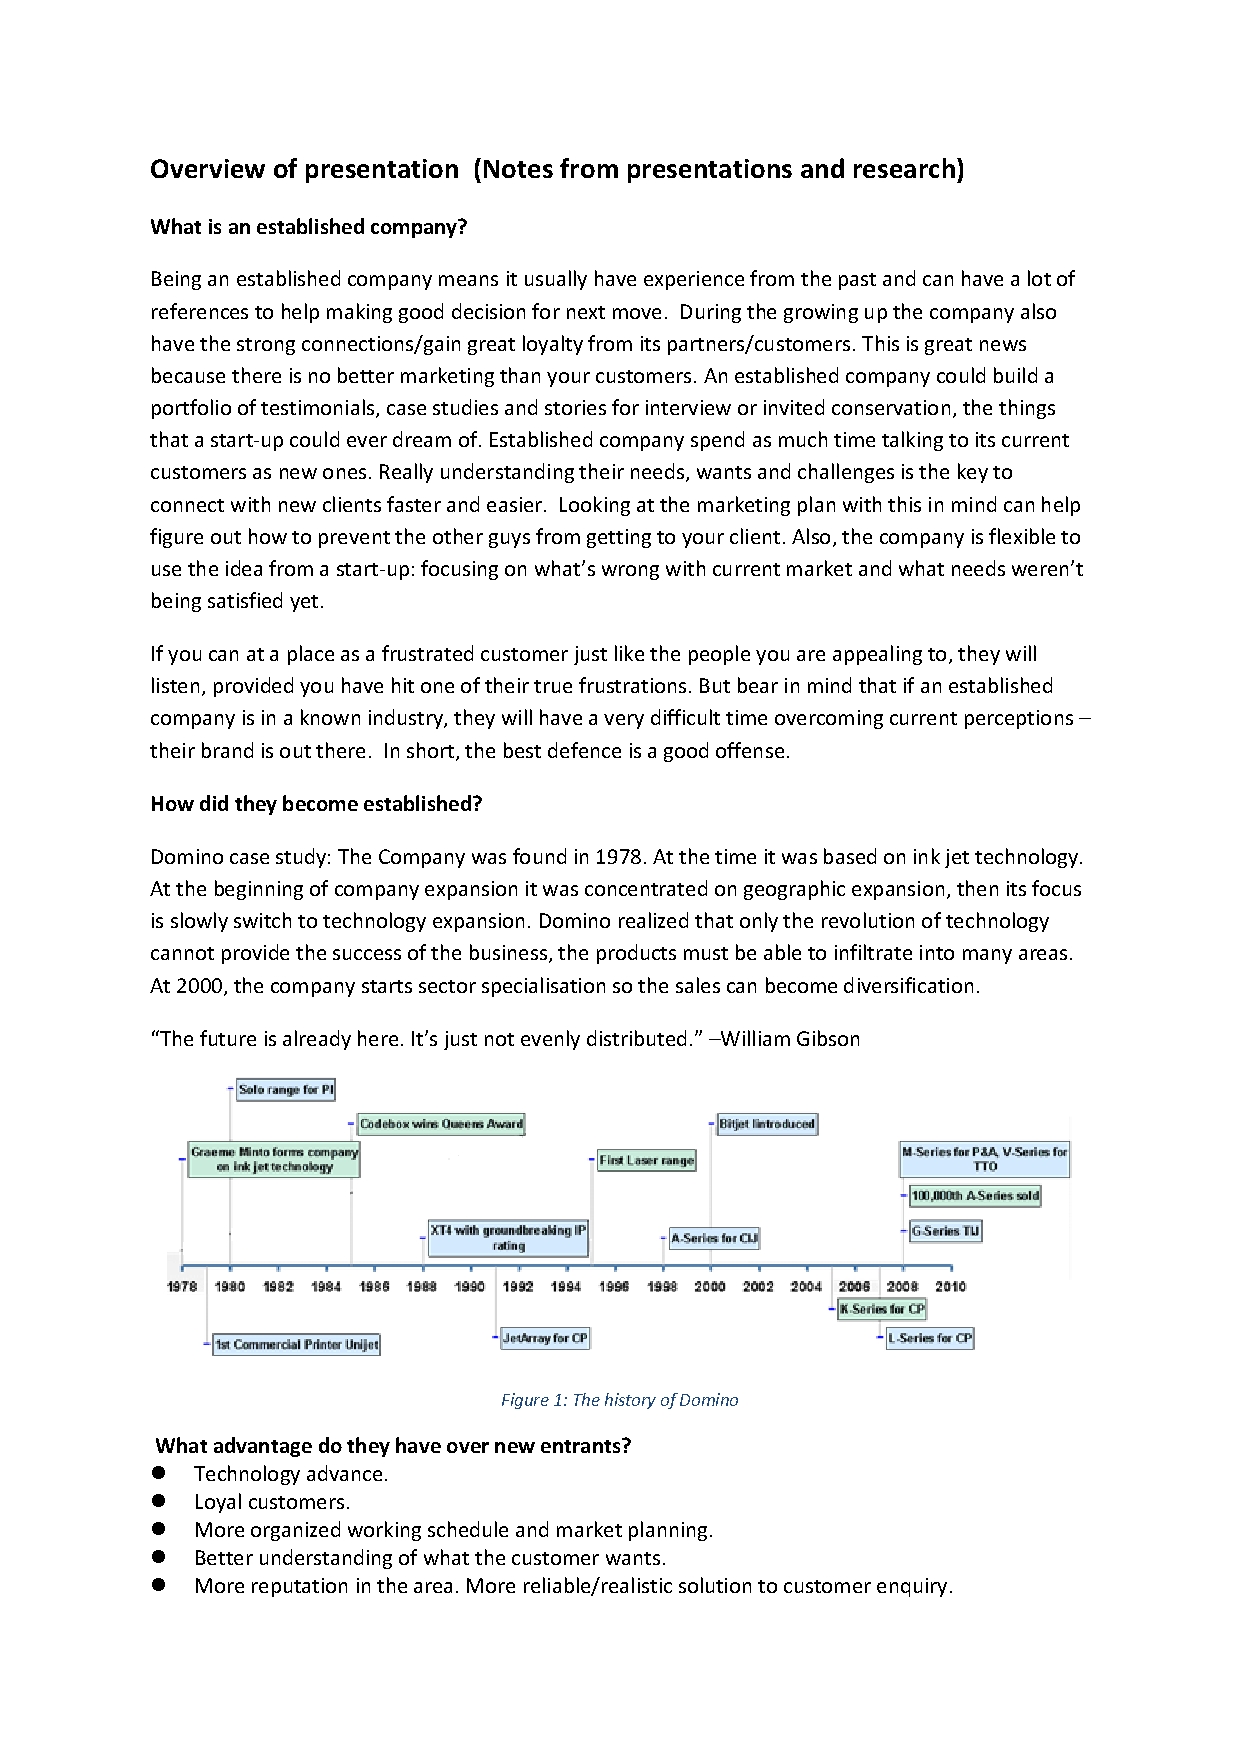
\includegraphics[width = 0.9\textwidth]{Figures/Overview_of_presentations}
		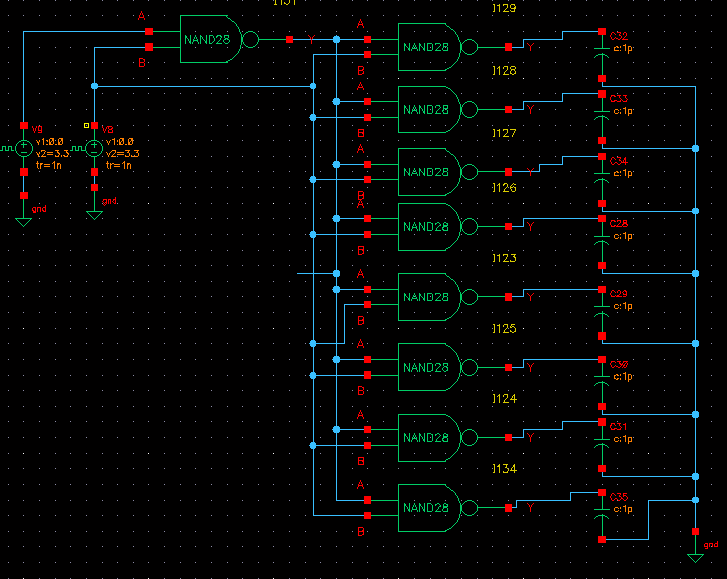
\includegraphics[width = 0.7\textwidth]{Figures/nandtest1}		
		\caption{NAND28 test circuit}
		\label {fig:nandtest1}
\end{figure*}

The result (Figure~\ref{fig:good}) shows that the NAND gate design is functioning properly with input signal at 100Mhz. The rise up time is approximate 8ns, which is similar to general manufactured NANDs in the industry~\cite{}~\cite{}. Further decreasing the width of transistors will cause output signal fail to reach the voltage level on time, as shown in Figure~\ref{fig:bad}

\begin{figure}[H]
		\centering
		%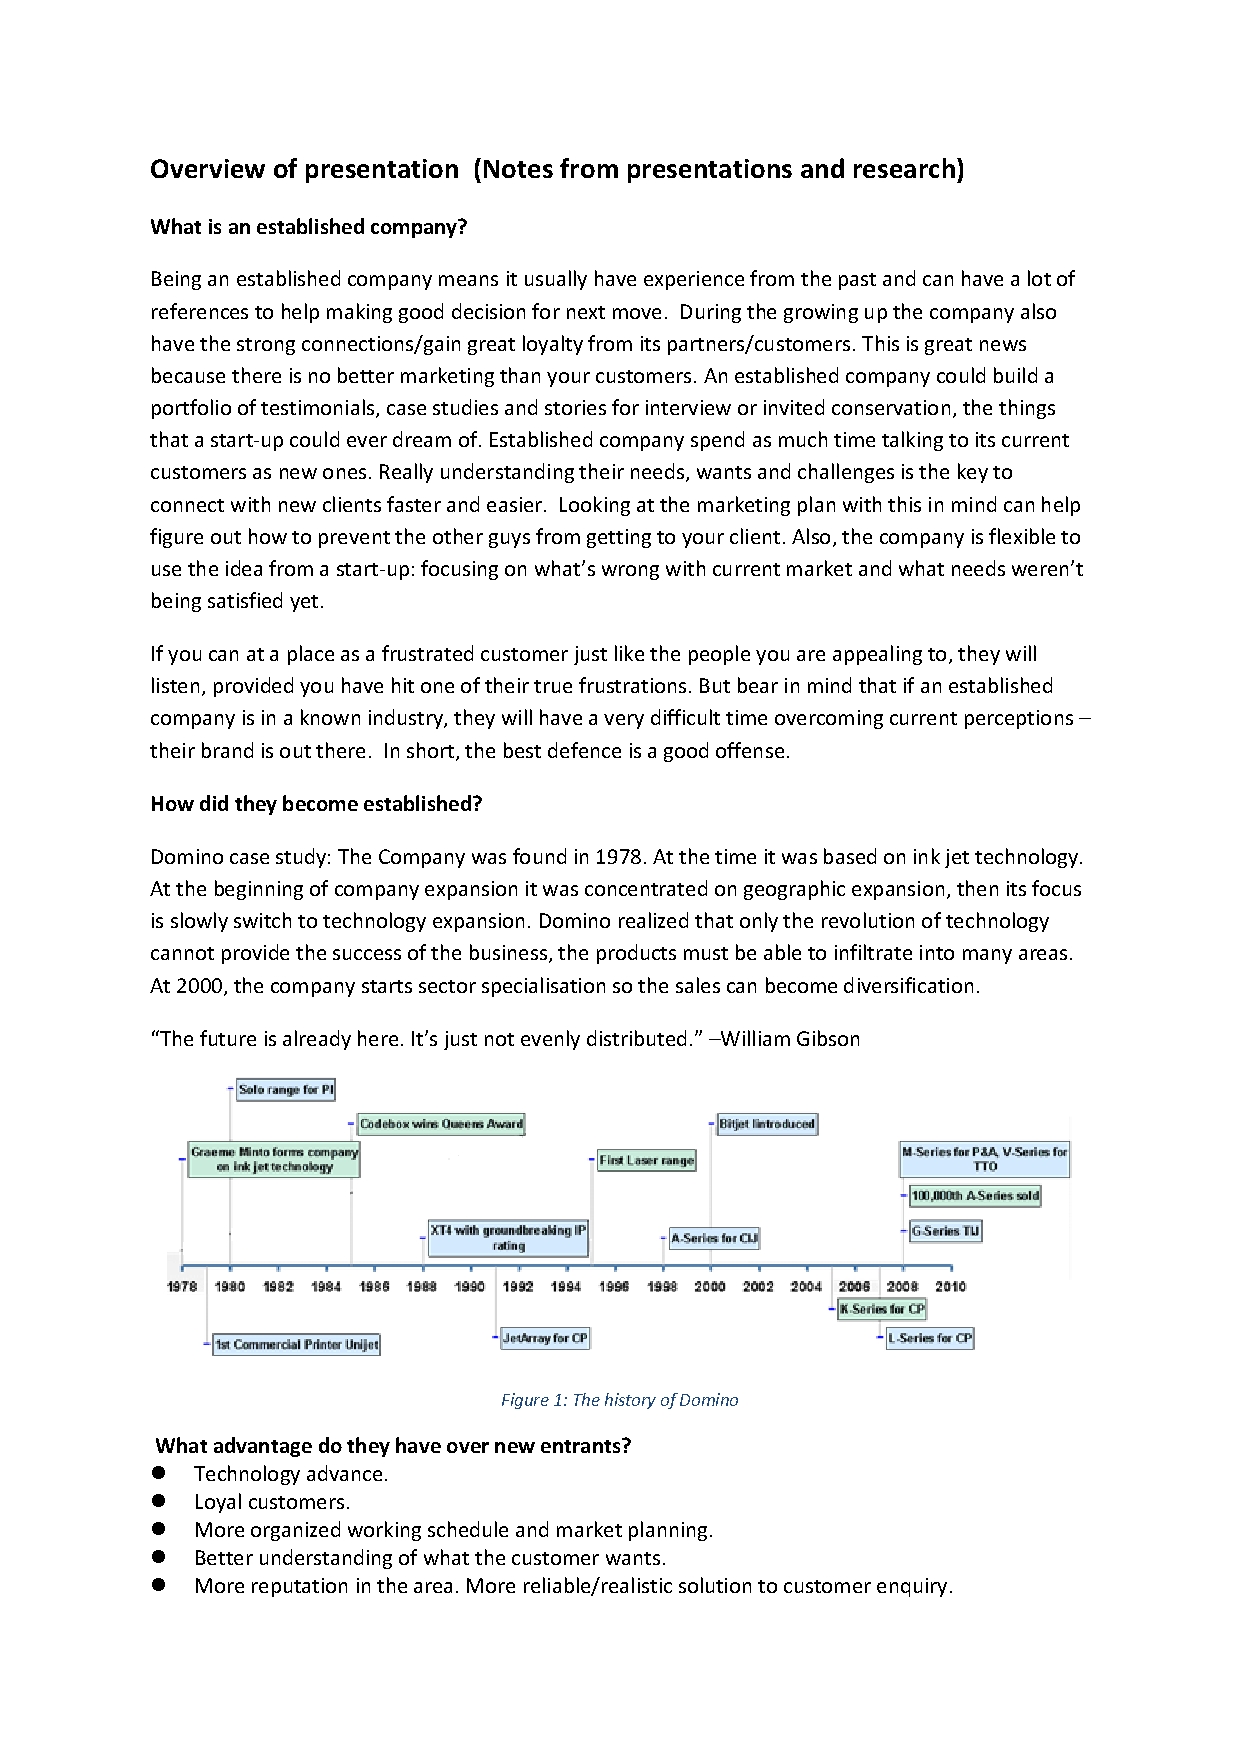
\includegraphics[width = 0.9\textwidth]{Figures/Overview_of_presentations}
		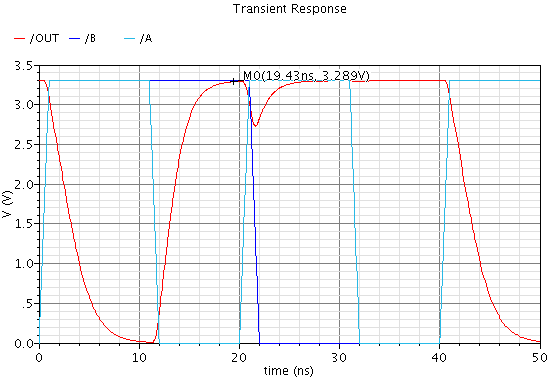
\includegraphics[width = 0.45\textwidth]{Figures/good}		
		\caption{Correct function of NAND gate}
		\label {fig:good}
\end{figure}

\begin{figure}[H]
		\centering
		%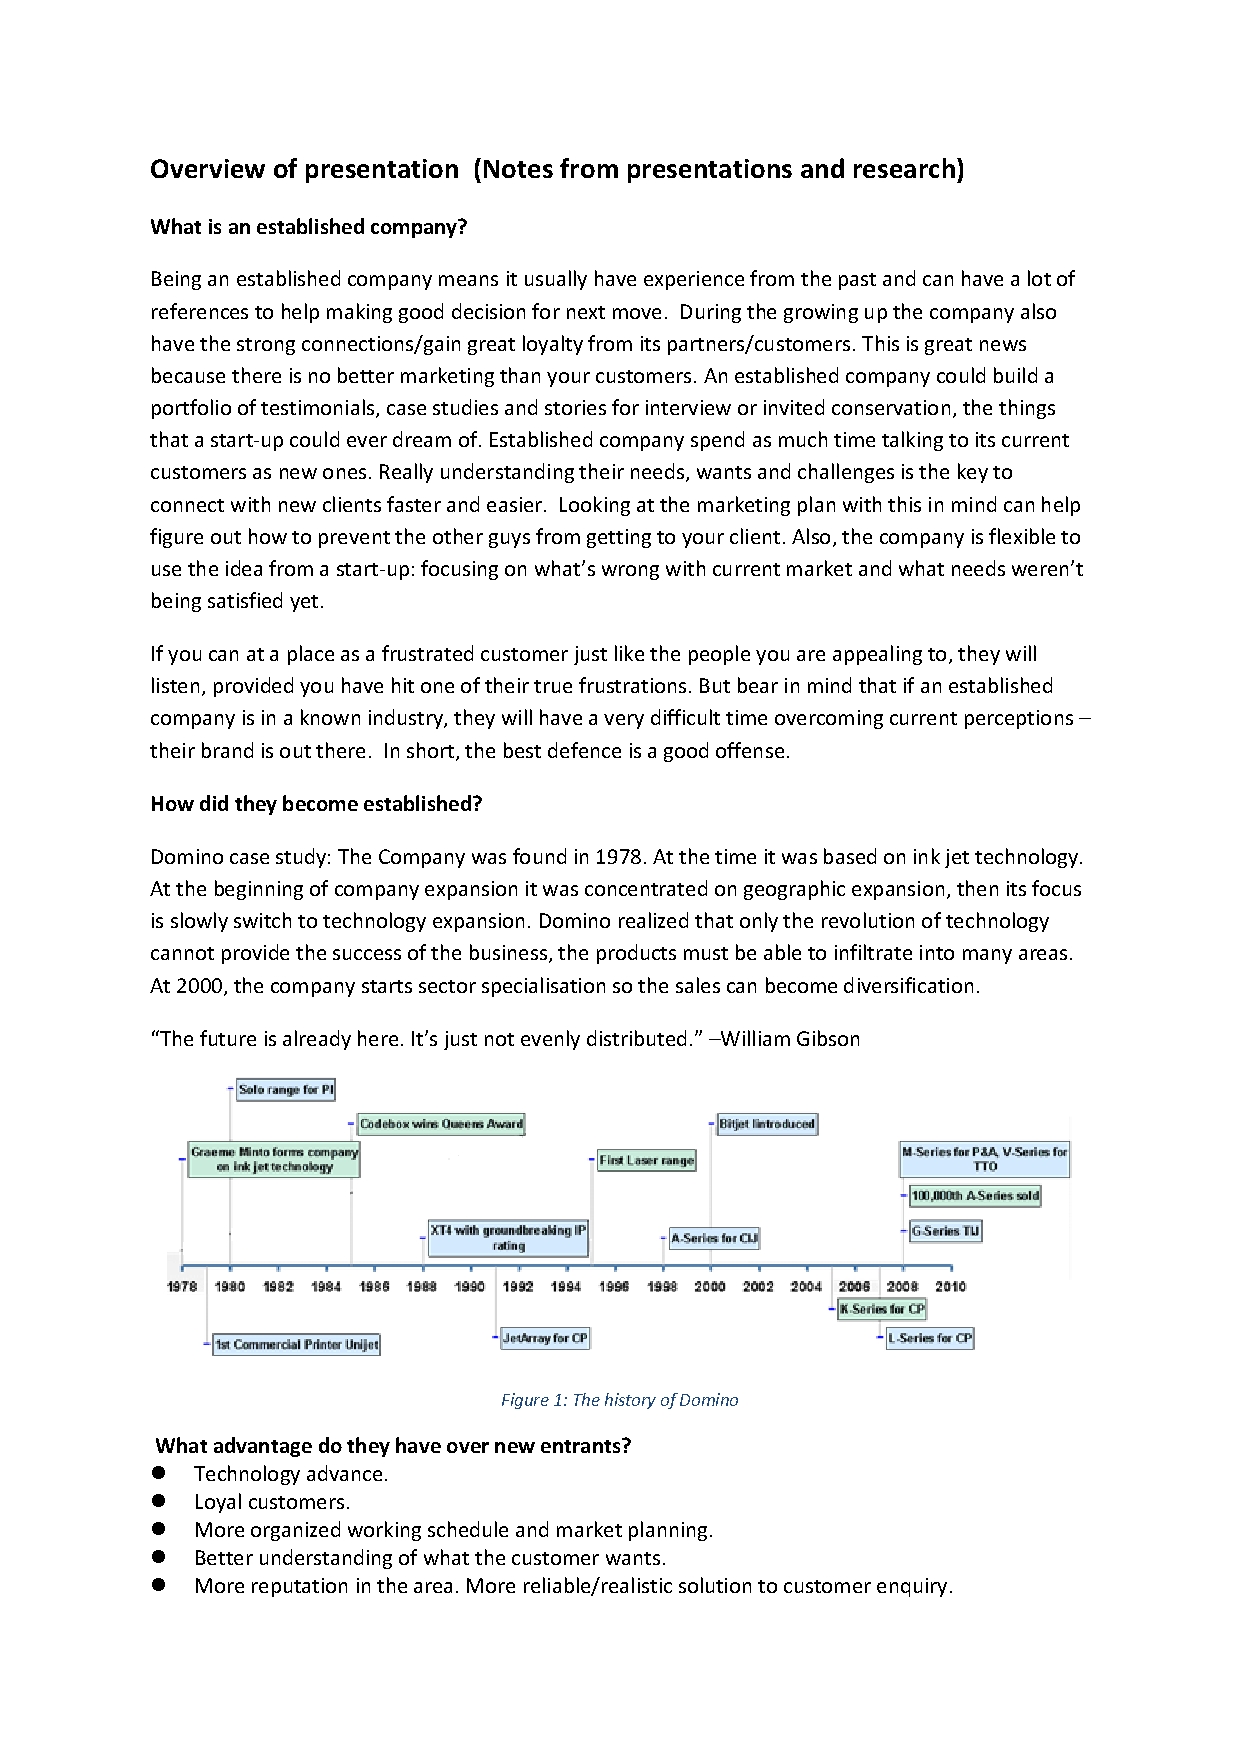
\includegraphics[width = 0.9\textwidth]{Figures/Overview_of_presentations}
		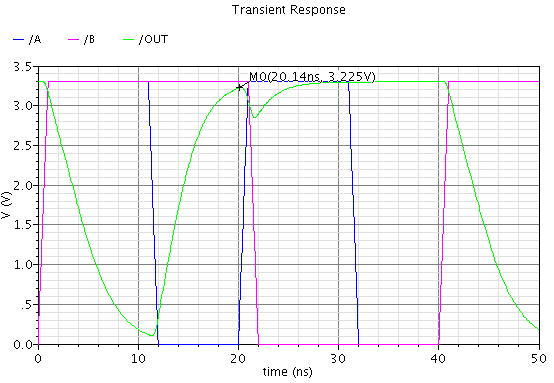
\includegraphics[width = 0.45\textwidth]{Figures/BAD}		
		\caption{NAND gate is too slow}
		\label {fig:bad}
\end{figure}